\section{Gestion des droits}

\section*{Responsable}

\begin{center}
\scalebox{0.7}{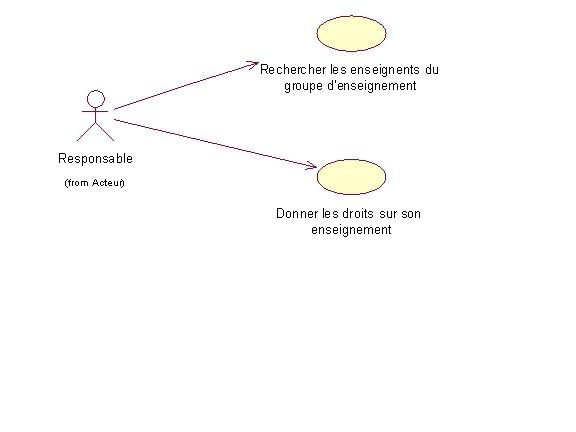
\includegraphics{images/Droits_Responsable.jpg}}\\
\end{center}

\begin{tabular}{|p{4cm}|c|p{4cm}|p{5cm}|}
\hline
  Fonction & Priorit{\'e} & Qualit{\'e} & Mesure \\
\hline
Rechercher les enseignants du groupe d'enseignement & 3 &  pr{\'e}cis & la recherche doit {\^e}tre pr{\'e}cis pour trouver l'{\'e}l{\'e}ment recherch{\'e} rapidement\\
\hline
Donner les droits sur un enseignement & 2 & sur & les droits doivent {\^e}tre donn{\'e}s sans erreurs\\
\hline
\end{tabular}

\begin{center}
{\'e}chelle de mesure de la priorit{\'e}:
\scalebox{0.5}{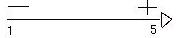
\includegraphics{images/echelle.jpg}}
\end{center}

\begin{itemize}	
\item {\bf Rechercher les enseignants du groupe d'enseignement :}
	\begin{itemize}
	\item Pr{\'e}-requis : {\^e}tre loger en tant que responsable.
	\item Description : L'utilisateur clique sur le lien {\it Rechercher enseignant}.\\
	Il donne aux choix avec ou sans crit{\`e}res qui donne une liste des enseignants qui appartiennent au groupe d'enseignement choisit.
	\item Post-requis : La liste est affich{\'e}e.\\
	\end{itemize}
\item {\bf Donner les droits sur un enseignement:}
	\begin{itemize}
	\item Pr{\'e}-requis : Etre identifi{\'e}/log{\'e} comme responsable de l'enseignement qu'il va modifier.\\
	Avoir list{\'e} avant tous les enseignants qui veut mettre en responsable de l'enseignement. 
	\item Description : Il ajoute � son enseignement des enseignant qui deviennent responsables eux aussi de cet enseignement.
	\item Post-requis : Des droits ont {\'e}t{\'e}s donn{\'e}s {\`a} d'autres enseignements que le cr{\'e}ateur.\\
	\end{itemize}
\end{itemize}

\section*{Administrateur}

\begin{center}
\scalebox{0.7}{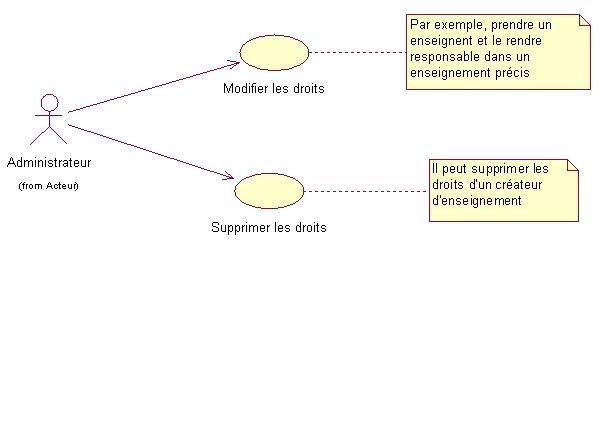
\includegraphics{images/Droits_Administrateur.jpg}}\\
\end{center}

\begin{tabular}{|p{4cm}|c|p{4cm}|p{5cm}|}
\hline
  Fonction & Priorit{\'e} & Qualit{\'e} & Mesure \\
\hline
Modifier les droits & 2 & fiable et s�r & \\
\hline
Supprimer les droits & 2 & fiable &\\
\hline
\end{tabular}

\begin{center}
{\'e}chelle de mesure de la priorit{\'e}:

\scalebox{0.5}{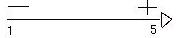
\includegraphics{images/echelle.jpg}}
\end{center}

\begin{itemize}
\item {\bf Modifier les droits :}
	\begin{itemize}
	\item Pr{\'e}-requis : Etre identifi{\'e}/log{\'e}. 
	\item Description : L'administrateur va modifier les droits des responsables.\\
	Il peut retirer le droit � un responsable et le faire donc passer simple enseignant et il peut faire passer un enseignant en responsable.
	\item Post-requis : Les modifications ont {\'e}t{\'e} effectu{\'e}es et sauvegard{\'e}es.\\
	\end{itemize}
\item {\bf Supprimer les droits :}
	\begin{itemize}
	\item Pr{\'e}-requis : Etre identifi{\'e}/log{\'e}. 
	\item Description : L'administrateur va supprimer les droits des responsables e il peut supprimer le droit � un responsable et le faire donc passer simple enseignant.
	\item Post-requis : Les modifications ont {\'e}t{\'e} effectu{\'e}es et sauvegard{\'e}es.\\
	\end{itemize}
\end{itemize}
